\documentclass[a4paper,twoside]{book}
\usepackage{graphicx}
\usepackage{url}
\usepackage{siunitx}
\usepackage{harvard}
\usepackage{GoudyIn,lettrine}
\renewcommand\LettrineFontHook{\GoudyInfamily}
\newcommand{\URL}[1]{$\langle$\url{#1}$\rangle$}
% This is the chapter titled `Optical TEMPEST' in Ireneusz Kubiak's new book.
\begin{document}
\title{New Book}
\author{Joe Loughry}
\setcounter{chapter}{6} % This chapter will be Chapter 7 of the book.
\setcounter{page}{99} % Arbitrary page number to test page numbering.
\chapter{Optical TEMPEST}
\lettrine[lines=3]{T}{he} leakage of information from a system through a
channel of modulated light is a vulnerability. The operative terms are `leakage',
`information', `channel', and `modulated light'. \emph{Leakage} might be
accidental or it might be caused on purpose by an adversary, but it is not
supposed to be there. \emph{Information} can be anything from a single bit to
large volumes of information; it might be extremely valuable information like
cryptographic keys. \emph{Channels} in the Shannon sense\cite{Shannon1948}
have a bandwidth-delay product, and noise; both of these are important to
understand the risk of optical TEMPEST. And finally, \emph{modulated light}
carries the signal. Light can be modulated in time or in space---here we think of
light modulated in the time domain. Light modulated in the space domain is an
\emph{image}; `shoulder surfing' is a real risk but not the one we are
concerned with here.

Further in the time domain, light can be amplitude-modulated, or frequency, or
phase. Of the three possibilities, amplitude modulation (AM) is the most
plausible, from a physical standpoint, because optical TEMPEST most often
depends on the accidental existence of a modulated---or modulatable---channel,
and AM is the simplest and most straightforward to implement.

on-off keying (OOK) b/c accidental; the adversary must exploit what's there
Manchester, if deliberate

Depending on the nature of the leakage, information leakage through optical
emanations may or may not be a covert channel. By the classical definition,
due to \cite{Lampson1973}, a covert channel is made of a pair of communicating
processes, but in many cases, the source of compromising optical emanations
is in hardware, not a programme running on the CPU.

electromagnetic but in the optical spectrum; we consider that to include at
least infrared (wavelengths longer than \SI{700}{\nano\metre}) because of the
ubiquitousness of light emitting diode (LED) sources in that range and their
convenient invisibility to humans.

reiterate the Class I, II, III taxonomy

\section{History}
The U.S.\ National Security Agency (NSA) named TEMPEST, as far as we know. We
don't even know for sure that the word is not an acronym. It is believed to
be a code name, \textsc{Tempest}\footnote{Evidence for it is shaky but there
was supposedly another programme called \textsc{Teapot} dealing with
stimulated RF compromising emanations \cite[p.~539]{Anderson2008a} and
partially corroborated in December of 2013 by Edward Snowden (NSA ANT
catalogue).} but evidence in the open literature is scarce; the only clear
original source is one declassified document dating from 1972 in which
everything related to emanations other than RF is redacted
\cite{NSAtempest2007}.
\subsection{Information Leakage}
\subsubsection{Electromagnetic}
Field telephones in WWI; {\it funkspiel} in WWII; electromechanical cypher
machines in West Berlin. (This topic is covered well elsewhere in the book.)
\subsection{TEMPEST}
The protection of information from remote eavesdropping; air gaps; control
zones; protected distribution systems (PDS)\footnote{Visibility, stories of
poison gas, flammable gas, pressure gauges---reference Anderson (2001).} The
inclusion of acoustic but overlooking of optical, with the exception of
shoulder surfing. Contextual blindness?
\subsection{Optical}
LEDs and CRTs---Figure \ref{figure:slow-mo_guys_crt}.
\begin{figure}[ht]
  \centering
  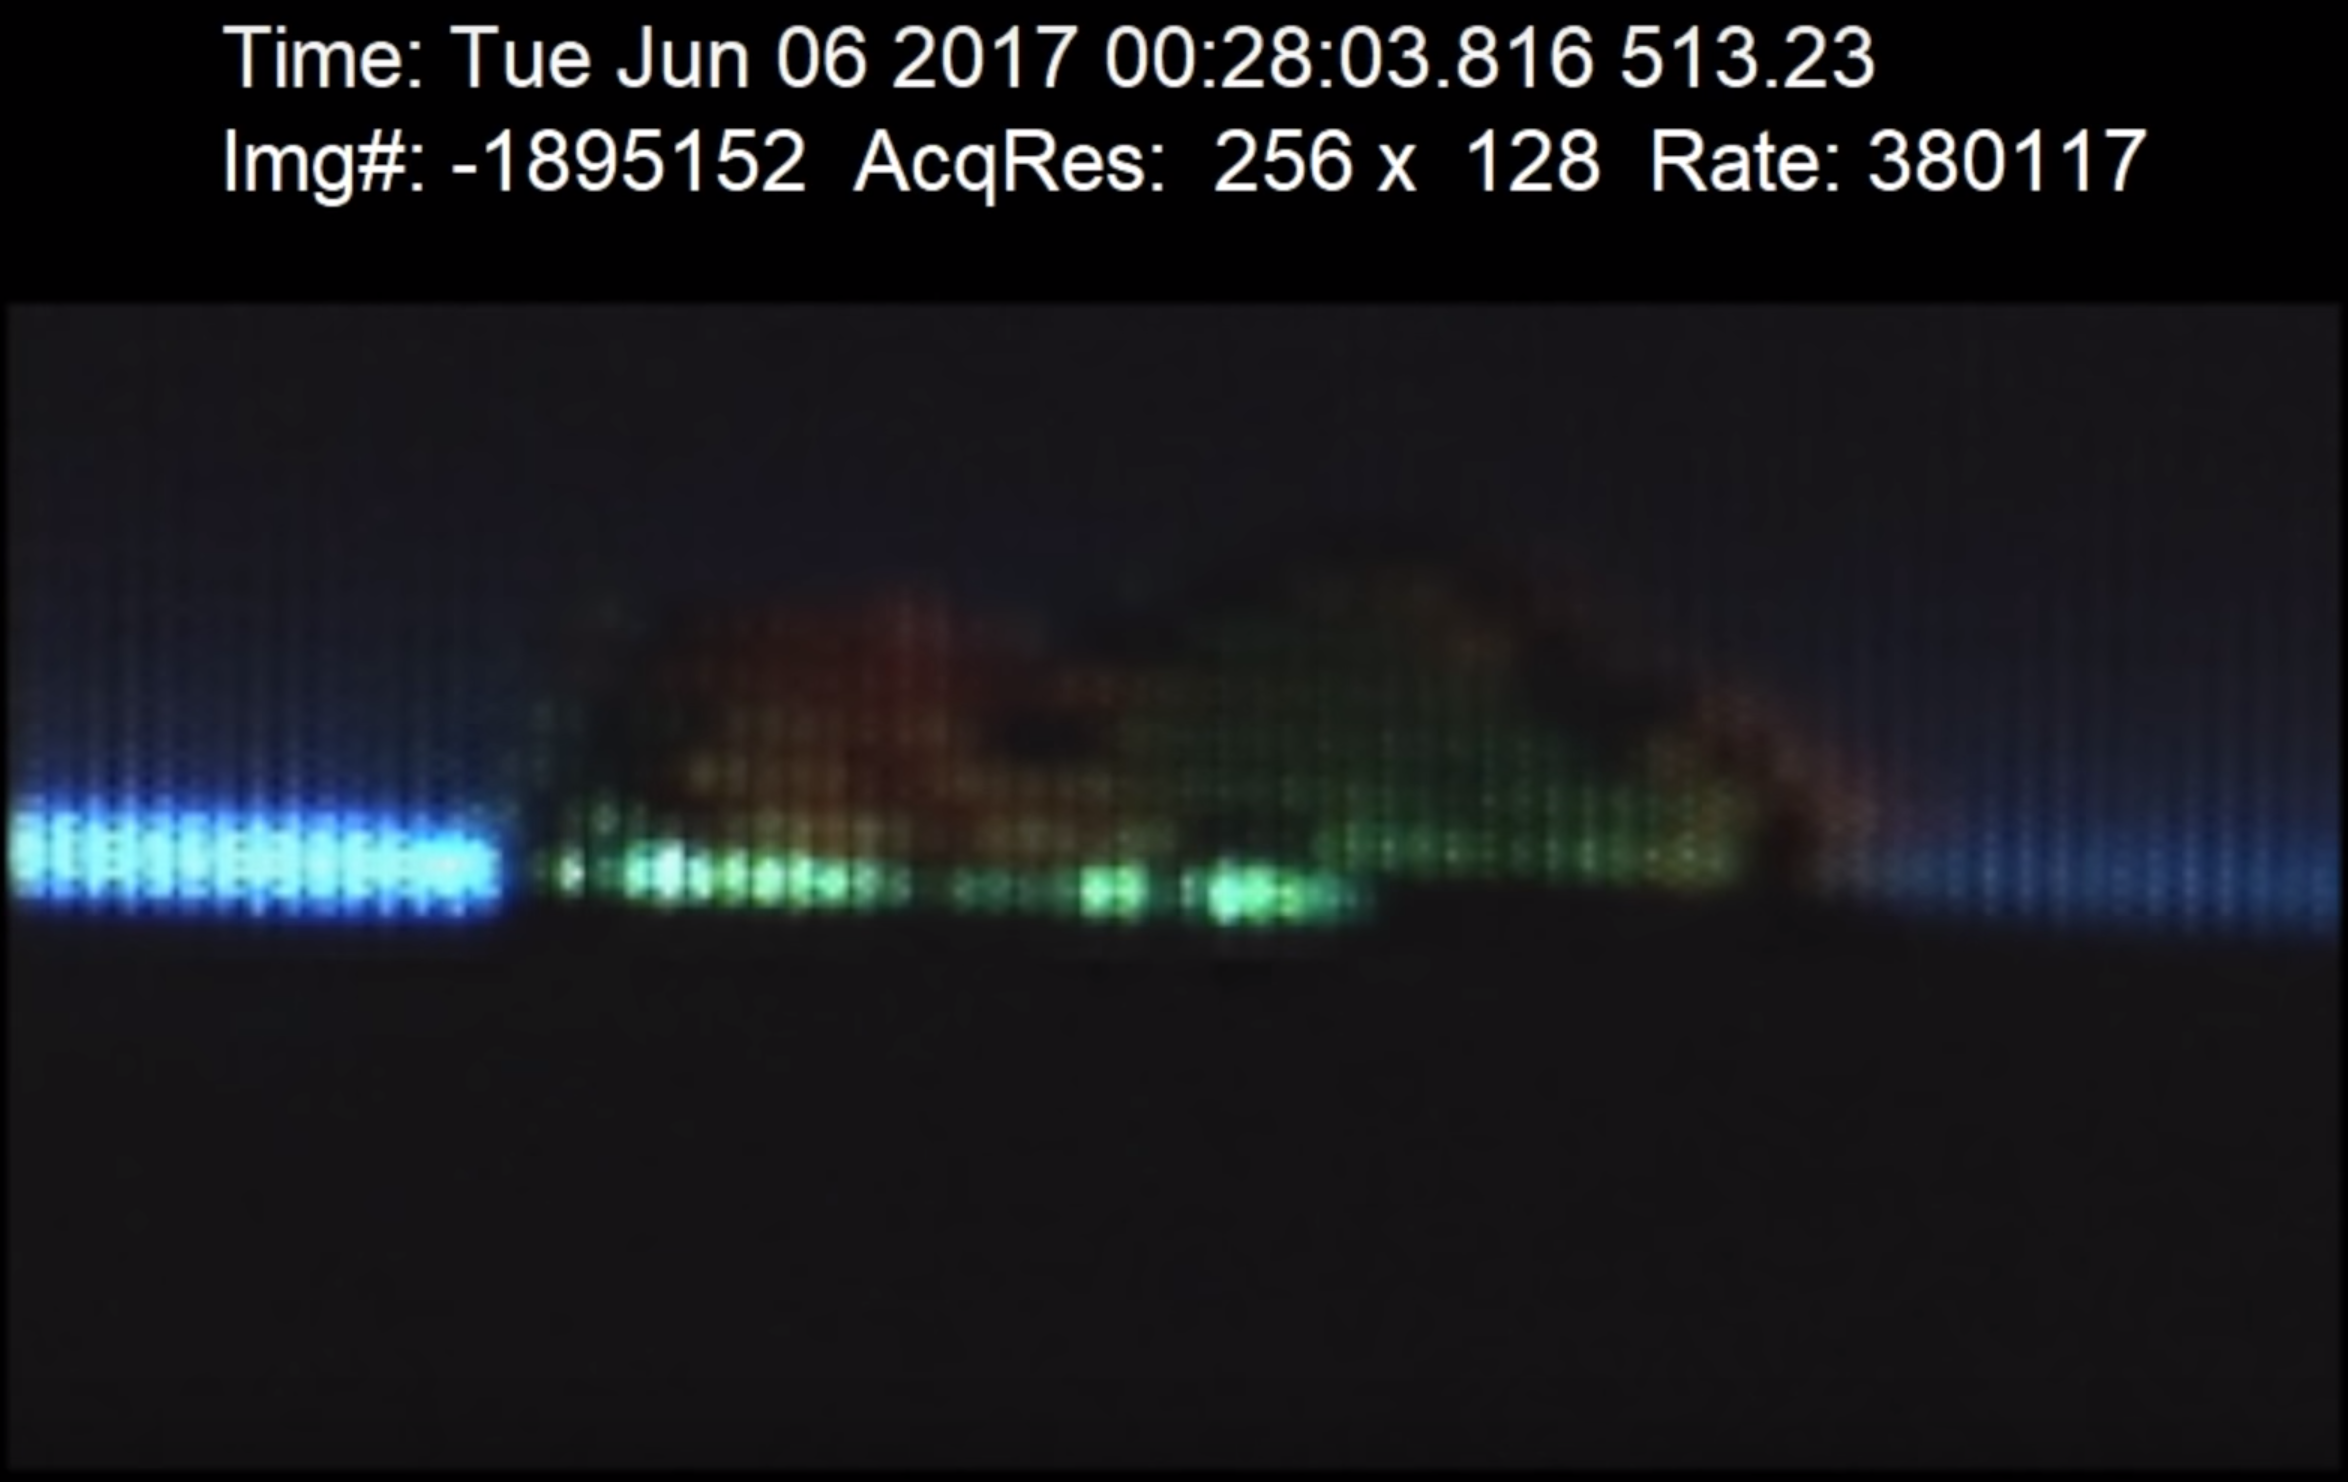
\includegraphics[width=3in]{slow-mo_guys_crt.png}
  \caption{High speed camera image (380\,117 frames per second) of CRT electron
    beam exciting phosphor dots \protect\cite{Free2018}.}
  \label{figure:slow-mo_guys_crt}
\end{figure}
\section{Physical Principles}
Photons, energy, generation atmospheric absorption. Recent development of
high efficiency LEDs (and the unexpected effect that had on reversing LEDs).
Telescopic optics, fibreoptic collection.
\begin{figure}[ht]
  \centering
  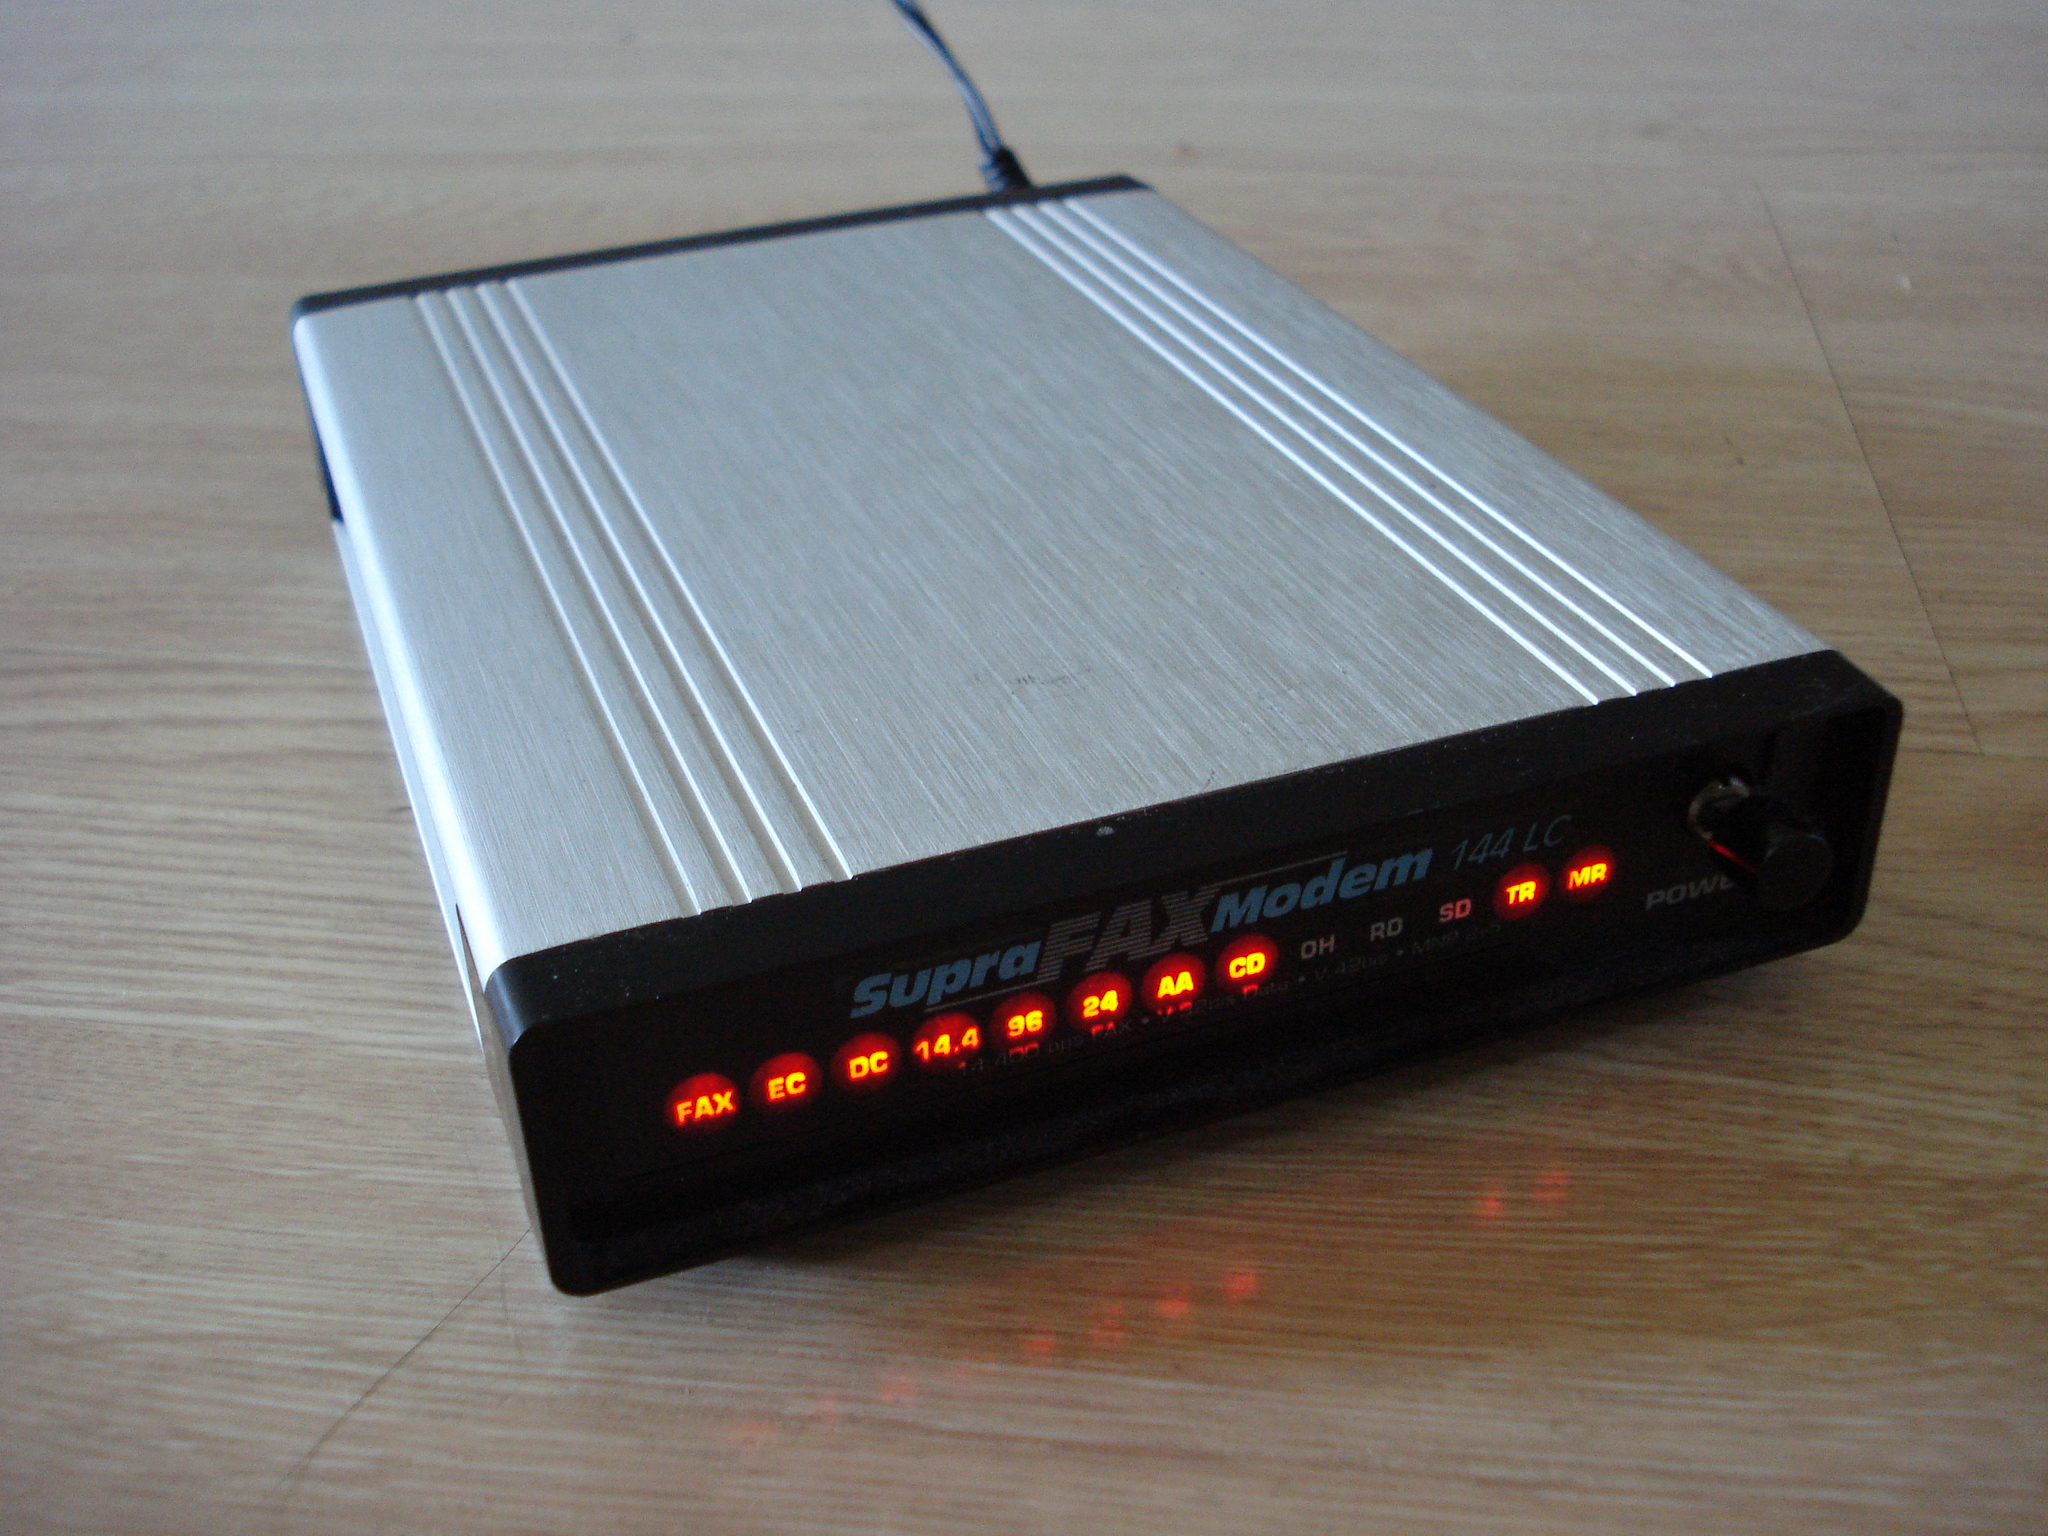
\includegraphics[width=3in]{SupraFAXmodem_144_LC_photo_courtesy_Wikipedia.jpg}
  \caption{Some LED indicators leak information.}
  \label{figure:modem}
\end{figure}
\subsection{The Unreasonable Effectiveness of Signal Processing}
One surprising thing, to anyone unfamiliar with digital signal processing, is
how effectively it can pull a usable signal out of what appears to be
hopelessly noisy data. An example may be seen in Fig.\ 4 of
\cite{Loughry2002a}.

Need a new figure here.

\section{Current Research}
Guri {\it et al.} But they are covert channels. But these are covert
channels. Difference between covert channels and side channels
(ref.\ Kocher).
\subsection{Resurgence of Interest 201?--present}
Aside from the `Compromising Reflections' paper, not much happened until
around 2010, except for\ldots\footnote{Parts of this section was presented at
EMC Europe 2018, in Amsterdam, the Netherlands (\emph{International Symposium
and Exhibition on Electromagnetic Compatibility}), 27--30 August 2018
\cite{Loughry2018a}.}
\subsection{Perspective}
It's not only LEDs; and LEDs are not only used as status indicators; Figure:
\emph{all} the information channels in and out of a PC---or more accurately,
an information processing system. A new conception of control zone;
Robinson's `energy gap' concept and its applicability to crypto.
\section{Future Directions}
Unpublished research
\subsection{LED Reversing}
Recent research---as yet unpublished---extends the idea of information leakage
through LEDs in the other direction. Unintended photosensitivity of junction
semiconductor devices has been known since at least the nineteen-seventies;
UV-eraseable programmable read-only memory (EPROM) chips take advantage of the
fact. Mims \citeyear{Mims1973b} was first to note in print that LEDs work as
photodiodes, both in the forward-biased (photovoltaic) and reverse-biased
(photoconductive) modes.

Would an unmodified LED, with leads splayed out, act as a WiFi powered
optical bug? Could a \SI{5}{\giga\hertz} WiFi illumination power it in
\emph{reverse bias} photoconductive mode to turn it into an optical RF
modulator? It's a nonlinear junction (diode) detector already---but can
incident \emph{optical} radiation modulate through the diode the reflection
from the leads of the ambient microwave interrogation carrier?

Modern microprocessors do not expose their address and data bus lines as
earlier ones did. But what happens when LEDs on external pins (whether
configured for output, by the system designer, or reconfigured for input by an
attacker) drive those pins unexpectedly?

{\it Cf.}\ Snowden's disclosures of NSA's TAO catalogue, for a certainty.
\subsubsection{Classical covert channels}
\subsubsection{Dead blow hammer}
\bibliographystyle{agsm}
\bibliography{consolidated_bibtex_file}
\end{document}
